% Options for packages loaded elsewhere
\PassOptionsToPackage{unicode}{hyperref}
\PassOptionsToPackage{hyphens}{url}
\PassOptionsToPackage{dvipsnames,svgnames,x11names}{xcolor}
%
\documentclass[
  letterpaper,
  DIV=11,
  numbers=noendperiod]{scrartcl}

\usepackage{amsmath,amssymb}
\usepackage{iftex}
\ifPDFTeX
  \usepackage[T1]{fontenc}
  \usepackage[utf8]{inputenc}
  \usepackage{textcomp} % provide euro and other symbols
\else % if luatex or xetex
  \usepackage{unicode-math}
  \defaultfontfeatures{Scale=MatchLowercase}
  \defaultfontfeatures[\rmfamily]{Ligatures=TeX,Scale=1}
\fi
\usepackage{lmodern}
\ifPDFTeX\else  
    % xetex/luatex font selection
\fi
% Use upquote if available, for straight quotes in verbatim environments
\IfFileExists{upquote.sty}{\usepackage{upquote}}{}
\IfFileExists{microtype.sty}{% use microtype if available
  \usepackage[]{microtype}
  \UseMicrotypeSet[protrusion]{basicmath} % disable protrusion for tt fonts
}{}
\makeatletter
\@ifundefined{KOMAClassName}{% if non-KOMA class
  \IfFileExists{parskip.sty}{%
    \usepackage{parskip}
  }{% else
    \setlength{\parindent}{0pt}
    \setlength{\parskip}{6pt plus 2pt minus 1pt}}
}{% if KOMA class
  \KOMAoptions{parskip=half}}
\makeatother
\usepackage{xcolor}
\setlength{\emergencystretch}{3em} % prevent overfull lines
\setcounter{secnumdepth}{-\maxdimen} % remove section numbering
% Make \paragraph and \subparagraph free-standing
\ifx\paragraph\undefined\else
  \let\oldparagraph\paragraph
  \renewcommand{\paragraph}[1]{\oldparagraph{#1}\mbox{}}
\fi
\ifx\subparagraph\undefined\else
  \let\oldsubparagraph\subparagraph
  \renewcommand{\subparagraph}[1]{\oldsubparagraph{#1}\mbox{}}
\fi

\usepackage{color}
\usepackage{fancyvrb}
\newcommand{\VerbBar}{|}
\newcommand{\VERB}{\Verb[commandchars=\\\{\}]}
\DefineVerbatimEnvironment{Highlighting}{Verbatim}{commandchars=\\\{\}}
% Add ',fontsize=\small' for more characters per line
\usepackage{framed}
\definecolor{shadecolor}{RGB}{241,243,245}
\newenvironment{Shaded}{\begin{snugshade}}{\end{snugshade}}
\newcommand{\AlertTok}[1]{\textcolor[rgb]{0.68,0.00,0.00}{#1}}
\newcommand{\AnnotationTok}[1]{\textcolor[rgb]{0.37,0.37,0.37}{#1}}
\newcommand{\AttributeTok}[1]{\textcolor[rgb]{0.40,0.45,0.13}{#1}}
\newcommand{\BaseNTok}[1]{\textcolor[rgb]{0.68,0.00,0.00}{#1}}
\newcommand{\BuiltInTok}[1]{\textcolor[rgb]{0.00,0.23,0.31}{#1}}
\newcommand{\CharTok}[1]{\textcolor[rgb]{0.13,0.47,0.30}{#1}}
\newcommand{\CommentTok}[1]{\textcolor[rgb]{0.37,0.37,0.37}{#1}}
\newcommand{\CommentVarTok}[1]{\textcolor[rgb]{0.37,0.37,0.37}{\textit{#1}}}
\newcommand{\ConstantTok}[1]{\textcolor[rgb]{0.56,0.35,0.01}{#1}}
\newcommand{\ControlFlowTok}[1]{\textcolor[rgb]{0.00,0.23,0.31}{#1}}
\newcommand{\DataTypeTok}[1]{\textcolor[rgb]{0.68,0.00,0.00}{#1}}
\newcommand{\DecValTok}[1]{\textcolor[rgb]{0.68,0.00,0.00}{#1}}
\newcommand{\DocumentationTok}[1]{\textcolor[rgb]{0.37,0.37,0.37}{\textit{#1}}}
\newcommand{\ErrorTok}[1]{\textcolor[rgb]{0.68,0.00,0.00}{#1}}
\newcommand{\ExtensionTok}[1]{\textcolor[rgb]{0.00,0.23,0.31}{#1}}
\newcommand{\FloatTok}[1]{\textcolor[rgb]{0.68,0.00,0.00}{#1}}
\newcommand{\FunctionTok}[1]{\textcolor[rgb]{0.28,0.35,0.67}{#1}}
\newcommand{\ImportTok}[1]{\textcolor[rgb]{0.00,0.46,0.62}{#1}}
\newcommand{\InformationTok}[1]{\textcolor[rgb]{0.37,0.37,0.37}{#1}}
\newcommand{\KeywordTok}[1]{\textcolor[rgb]{0.00,0.23,0.31}{#1}}
\newcommand{\NormalTok}[1]{\textcolor[rgb]{0.00,0.23,0.31}{#1}}
\newcommand{\OperatorTok}[1]{\textcolor[rgb]{0.37,0.37,0.37}{#1}}
\newcommand{\OtherTok}[1]{\textcolor[rgb]{0.00,0.23,0.31}{#1}}
\newcommand{\PreprocessorTok}[1]{\textcolor[rgb]{0.68,0.00,0.00}{#1}}
\newcommand{\RegionMarkerTok}[1]{\textcolor[rgb]{0.00,0.23,0.31}{#1}}
\newcommand{\SpecialCharTok}[1]{\textcolor[rgb]{0.37,0.37,0.37}{#1}}
\newcommand{\SpecialStringTok}[1]{\textcolor[rgb]{0.13,0.47,0.30}{#1}}
\newcommand{\StringTok}[1]{\textcolor[rgb]{0.13,0.47,0.30}{#1}}
\newcommand{\VariableTok}[1]{\textcolor[rgb]{0.07,0.07,0.07}{#1}}
\newcommand{\VerbatimStringTok}[1]{\textcolor[rgb]{0.13,0.47,0.30}{#1}}
\newcommand{\WarningTok}[1]{\textcolor[rgb]{0.37,0.37,0.37}{\textit{#1}}}

\providecommand{\tightlist}{%
  \setlength{\itemsep}{0pt}\setlength{\parskip}{0pt}}\usepackage{longtable,booktabs,array}
\usepackage{calc} % for calculating minipage widths
% Correct order of tables after \paragraph or \subparagraph
\usepackage{etoolbox}
\makeatletter
\patchcmd\longtable{\par}{\if@noskipsec\mbox{}\fi\par}{}{}
\makeatother
% Allow footnotes in longtable head/foot
\IfFileExists{footnotehyper.sty}{\usepackage{footnotehyper}}{\usepackage{footnote}}
\makesavenoteenv{longtable}
\usepackage{graphicx}
\makeatletter
\def\maxwidth{\ifdim\Gin@nat@width>\linewidth\linewidth\else\Gin@nat@width\fi}
\def\maxheight{\ifdim\Gin@nat@height>\textheight\textheight\else\Gin@nat@height\fi}
\makeatother
% Scale images if necessary, so that they will not overflow the page
% margins by default, and it is still possible to overwrite the defaults
% using explicit options in \includegraphics[width, height, ...]{}
\setkeys{Gin}{width=\maxwidth,height=\maxheight,keepaspectratio}
% Set default figure placement to htbp
\makeatletter
\def\fps@figure{htbp}
\makeatother

\usepackage{fvextra}
\DefineVerbatimEnvironment{Highlighting}{Verbatim}{breaklines,commandchars=\\\{\}}
\DefineVerbatimEnvironment{OutputCode}{Verbatim}{breaklines,commandchars=\\\{\}}
\KOMAoption{captions}{tableheading}
\makeatletter
\makeatother
\makeatletter
\makeatother
\makeatletter
\@ifpackageloaded{caption}{}{\usepackage{caption}}
\AtBeginDocument{%
\ifdefined\contentsname
  \renewcommand*\contentsname{Table of contents}
\else
  \newcommand\contentsname{Table of contents}
\fi
\ifdefined\listfigurename
  \renewcommand*\listfigurename{List of Figures}
\else
  \newcommand\listfigurename{List of Figures}
\fi
\ifdefined\listtablename
  \renewcommand*\listtablename{List of Tables}
\else
  \newcommand\listtablename{List of Tables}
\fi
\ifdefined\figurename
  \renewcommand*\figurename{Figure}
\else
  \newcommand\figurename{Figure}
\fi
\ifdefined\tablename
  \renewcommand*\tablename{Table}
\else
  \newcommand\tablename{Table}
\fi
}
\@ifpackageloaded{float}{}{\usepackage{float}}
\floatstyle{ruled}
\@ifundefined{c@chapter}{\newfloat{codelisting}{h}{lop}}{\newfloat{codelisting}{h}{lop}[chapter]}
\floatname{codelisting}{Listing}
\newcommand*\listoflistings{\listof{codelisting}{List of Listings}}
\makeatother
\makeatletter
\@ifpackageloaded{caption}{}{\usepackage{caption}}
\@ifpackageloaded{subcaption}{}{\usepackage{subcaption}}
\makeatother
\makeatletter
\@ifpackageloaded{tcolorbox}{}{\usepackage[skins,breakable]{tcolorbox}}
\makeatother
\makeatletter
\@ifundefined{shadecolor}{\definecolor{shadecolor}{rgb}{.97, .97, .97}}
\makeatother
\makeatletter
\makeatother
\makeatletter
\makeatother
\ifLuaTeX
  \usepackage{selnolig}  % disable illegal ligatures
\fi
\IfFileExists{bookmark.sty}{\usepackage{bookmark}}{\usepackage{hyperref}}
\IfFileExists{xurl.sty}{\usepackage{xurl}}{} % add URL line breaks if available
\urlstyle{same} % disable monospaced font for URLs
\hypersetup{
  pdftitle={NIFB22001U Introduction to Econometrics Exam 2022/2023 - R Code Attachment},
  pdfauthor={Abdullah Faqih Al Mubarok},
  colorlinks=true,
  linkcolor={blue},
  filecolor={Maroon},
  citecolor={Blue},
  urlcolor={Blue},
  pdfcreator={LaTeX via pandoc}}

\title{NIFB22001U Introduction to Econometrics Exam 2022/2023 - R Code
Attachment}
\author{Abdullah Faqih Al Mubarok}
\date{}

\begin{document}
\maketitle
\ifdefined\Shaded\renewenvironment{Shaded}{\begin{tcolorbox}[interior hidden, frame hidden, borderline west={3pt}{0pt}{shadecolor}, sharp corners, enhanced, breakable, boxrule=0pt]}{\end{tcolorbox}}\fi

\begin{Shaded}
\begin{Highlighting}[]
\CommentTok{\#load libaries}
\FunctionTok{library}\NormalTok{(tidyverse)}
\FunctionTok{library}\NormalTok{(stargazer)}
\FunctionTok{library}\NormalTok{(lmtest)}
\FunctionTok{library}\NormalTok{(car)}
\FunctionTok{library}\NormalTok{(sandwich)}
\FunctionTok{library}\NormalTok{(AER)}
\FunctionTok{library}\NormalTok{(ggrepel)}
\FunctionTok{library}\NormalTok{(patchwork)}
\FunctionTok{library}\NormalTok{(corrplot)}


\CommentTok{\#load data }
\NormalTok{data\_01 }\OtherTok{\textless{}{-}} \FunctionTok{get}\NormalTok{(}\FunctionTok{load}\NormalTok{(}\StringTok{"examdata2023\_01.RData"}\NormalTok{))}
\NormalTok{data\_02 }\OtherTok{\textless{}{-}} \FunctionTok{get}\NormalTok{(}\FunctionTok{load}\NormalTok{(}\StringTok{"examdata2023\_02.RData"}\NormalTok{))}
\end{Highlighting}
\end{Shaded}

\hypertarget{part-1-the-returns-to-education}{%
\subsection{Part 1: The Returns to
Education}\label{part-1-the-returns-to-education}}

\begin{enumerate}
\def\labelenumi{\arabic{enumi}.}
\tightlist
\item
  Below code is used for estimating
\end{enumerate}

\begin{equation}
    \label{eq:1}
    wage = \alpha + \beta educ + u
  \end{equation}

\begin{Shaded}
\begin{Highlighting}[]
\NormalTok{model\_01\_pred }\OtherTok{\textless{}{-}} \FunctionTok{lm}\NormalTok{(}\AttributeTok{data =}\NormalTok{ data\_01, }
               \AttributeTok{formula =}\NormalTok{ wage }\SpecialCharTok{\textasciitilde{}}\NormalTok{ education)}

\CommentTok{\#Variance}
\FunctionTok{var}\NormalTok{(data\_01}\SpecialCharTok{$}\NormalTok{education)}

\FunctionTok{stargazer}\NormalTok{(model\_01\_pred, }\AttributeTok{type =} \StringTok{"text"}\NormalTok{)}
\end{Highlighting}
\end{Shaded}

\begin{enumerate}
\def\labelenumi{\arabic{enumi}.}
\setcounter{enumi}{1}
\tightlist
\item
  Covariance check between education and libraries
\end{enumerate}

\begin{Shaded}
\begin{Highlighting}[]
\FunctionTok{cov}\NormalTok{(data\_01}\SpecialCharTok{$}\NormalTok{education, data\_01}\SpecialCharTok{$}\NormalTok{libraries)}
\end{Highlighting}
\end{Shaded}

\begin{enumerate}
\def\labelenumi{\arabic{enumi}.}
\setcounter{enumi}{2}
\tightlist
\item
  2SLS regression of model (1)
\end{enumerate}

\begin{Shaded}
\begin{Highlighting}[]
\NormalTok{model\_01\_iv\_pred }\OtherTok{\textless{}{-}} \FunctionTok{ivreg}\NormalTok{(wage }\SpecialCharTok{\textasciitilde{}}\NormalTok{ education }\SpecialCharTok{|}\NormalTok{ libraries,}
                               \AttributeTok{data =}\NormalTok{ data\_01, }
                               \AttributeTok{model =} \ConstantTok{TRUE}\NormalTok{)}


\FunctionTok{stargazer}\NormalTok{(model\_01\_pred, model\_01\_iv\_pred, }\AttributeTok{type =} \StringTok{"text"}\NormalTok{)}
\end{Highlighting}
\end{Shaded}

\hypertarget{part-2-global-food-consumption-patterns}{%
\subsection{Part 2: Global Food Consumption
Patterns}\label{part-2-global-food-consumption-patterns}}

\hypertarget{data-description-and-preliminary-analysis}{%
\subsubsection{2.1 Data description and preliminary
analysis}\label{data-description-and-preliminary-analysis}}

\begin{enumerate}
\def\labelenumi{\arabic{enumi}.}
\tightlist
\item
  Descriptive statistic of supplied data
\end{enumerate}

\begin{Shaded}
\begin{Highlighting}[]
\FunctionTok{stargazer}\NormalTok{(data\_02, }\AttributeTok{type =} \StringTok{"text"}\NormalTok{, }\AttributeTok{median =} \ConstantTok{TRUE}\NormalTok{, }\AttributeTok{mean.sd =} \ConstantTok{TRUE}\NormalTok{, }\AttributeTok{digits =} \DecValTok{2}\NormalTok{)}
\end{Highlighting}
\end{Shaded}

\begin{enumerate}
\def\labelenumi{\arabic{enumi}.}
\setcounter{enumi}{1}
\tightlist
\item
  Consumption proportion vs GDP Per capita
\end{enumerate}

\begin{Shaded}
\begin{Highlighting}[]
\CommentTok{\#|warning : false}
\CommentTok{\#|eval: false}
\NormalTok{propcal\_gdp }\OtherTok{\textless{}{-}}\NormalTok{ data\_02 }\SpecialCharTok{|\textgreater{}} 
  \FunctionTok{select}\NormalTok{(Country, PropCalAnimal, PropCalVegetal, GdpPerCapita) }\SpecialCharTok{|\textgreater{}} 
  \FunctionTok{pivot\_longer}\NormalTok{(}\AttributeTok{cols =} \FunctionTok{starts\_with}\NormalTok{(}\StringTok{"PropCal"}\NormalTok{), }
               \AttributeTok{names\_to =} \StringTok{"ConsumType"}\NormalTok{, }\AttributeTok{values\_to =} \StringTok{"PropCal"}\NormalTok{)}

\FunctionTok{ggplot}\NormalTok{(}\AttributeTok{data =}\NormalTok{ propcal\_gdp, }
       \AttributeTok{mapping =} \FunctionTok{aes}\NormalTok{(}\AttributeTok{y =}\NormalTok{ PropCal, }\AttributeTok{x =}\NormalTok{ GdpPerCapita)) }\SpecialCharTok{+} 
  \FunctionTok{geom\_point}\NormalTok{(}\AttributeTok{color =} \StringTok{"blue"}\NormalTok{, }\AttributeTok{alpha =} \FloatTok{0.3}\NormalTok{) }\SpecialCharTok{+} 
  \FunctionTok{geom\_text\_repel}\NormalTok{(}\AttributeTok{size =} \DecValTok{2}\NormalTok{, }\AttributeTok{verbose =} \ConstantTok{FALSE}\NormalTok{,}
    \AttributeTok{mapping =} \FunctionTok{aes}\NormalTok{(}\AttributeTok{label =}\NormalTok{ Country)) }\SpecialCharTok{+} 
  \FunctionTok{facet\_grid}\NormalTok{(}\AttributeTok{rows =} \FunctionTok{vars}\NormalTok{(ConsumType), }\AttributeTok{scales =} \StringTok{"free"}\NormalTok{) }\SpecialCharTok{+}
  \FunctionTok{labs}\NormalTok{(}\AttributeTok{x =} \StringTok{"GdpPerCapita($)"}\NormalTok{) }\SpecialCharTok{+} 
  \FunctionTok{theme\_bw}\NormalTok{()}
\end{Highlighting}
\end{Shaded}

\begin{verbatim}
Warning: Removed 38 rows containing missing values (`geom_point()`).
\end{verbatim}

\begin{verbatim}
Warning: Removed 38 rows containing missing values (`geom_text_repel()`).
\end{verbatim}

\begin{verbatim}
Warning: ggrepel: 127 unlabeled data points (too many overlaps). Consider increasing max.overlaps
ggrepel: 127 unlabeled data points (too many overlaps). Consider increasing max.overlaps
\end{verbatim}

\begin{figure}[H]

{\centering 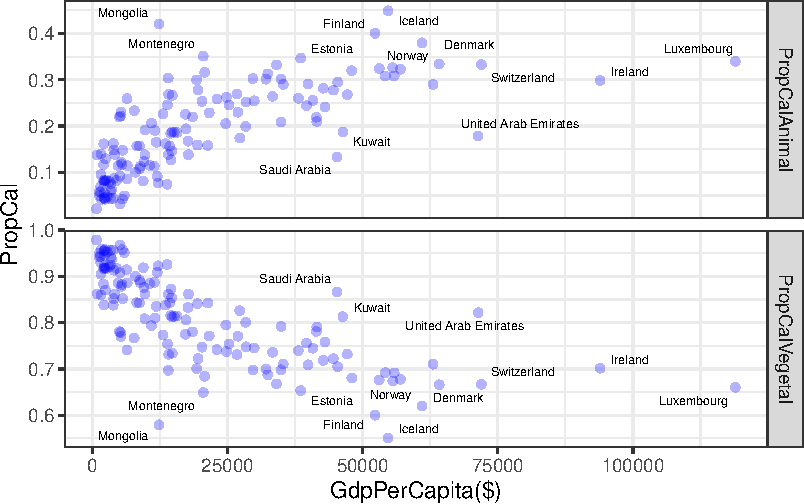
\includegraphics{code_files/figure-pdf/unnamed-chunk-6-1.pdf}

}

\end{figure}

\begin{enumerate}
\def\labelenumi{\arabic{enumi}.}
\setcounter{enumi}{1}
\tightlist
\item
  PropCalAnimal and log(PropCalAnimal) distribution
\end{enumerate}

\begin{Shaded}
\begin{Highlighting}[]
\CommentTok{\#|warning : false}
\CommentTok{\#|eval: false}

\CommentTok{\# Proceeding without missing values}
\NormalTok{data\_02 }\OtherTok{\textless{}{-}}\NormalTok{ data\_02 }\SpecialCharTok{|\textgreater{}} 
  \FunctionTok{filter}\NormalTok{(}\SpecialCharTok{!}\FunctionTok{is.na}\NormalTok{(PropCalAnimal))}

\NormalTok{PropCalAnimal\_dist }\OtherTok{\textless{}{-}}\NormalTok{ data\_02 }\SpecialCharTok{|\textgreater{}} 
  \FunctionTok{select}\NormalTok{(PropCalAnimal) }\SpecialCharTok{|\textgreater{}} 
  \FunctionTok{mutate}\NormalTok{(}\StringTok{"log(PropCalAnimal)"} \OtherTok{=} \FunctionTok{log}\NormalTok{(PropCalAnimal))}

\NormalTok{p1 }\OtherTok{\textless{}{-}} \FunctionTok{ggplot}\NormalTok{(}\AttributeTok{data =}\NormalTok{ PropCalAnimal\_dist, }
             \AttributeTok{mapping =} \FunctionTok{aes}\NormalTok{(}\AttributeTok{x =}\NormalTok{ PropCalAnimal)) }\SpecialCharTok{+}
  \FunctionTok{geom\_histogram}\NormalTok{(}\AttributeTok{mapping =} \FunctionTok{aes}\NormalTok{(}\AttributeTok{y =}\NormalTok{ ..density..), }
                 \AttributeTok{fill =} \StringTok{"lightblue"}\NormalTok{, }\AttributeTok{color =} \StringTok{"lightblue"}\NormalTok{,}
                 \AttributeTok{alpha =} \FloatTok{0.75}\NormalTok{) }\SpecialCharTok{+}
  \FunctionTok{geom\_density}\NormalTok{(}\AttributeTok{color =} \StringTok{"orange"}\NormalTok{) }\SpecialCharTok{+} 
  \FunctionTok{theme\_bw}\NormalTok{()}

\NormalTok{p2 }\OtherTok{\textless{}{-}} \FunctionTok{ggplot}\NormalTok{(}\AttributeTok{data =}\NormalTok{ PropCalAnimal\_dist, }
             \AttributeTok{mapping =} \FunctionTok{aes}\NormalTok{(}\AttributeTok{x =} \StringTok{\textasciigrave{}}\AttributeTok{log(PropCalAnimal)}\StringTok{\textasciigrave{}}\NormalTok{)) }\SpecialCharTok{+}
  \FunctionTok{geom\_histogram}\NormalTok{(}\AttributeTok{mapping =} \FunctionTok{aes}\NormalTok{(}\AttributeTok{y =}\NormalTok{ ..density..), }
                 \AttributeTok{fill =} \StringTok{"lightblue"}\NormalTok{, }\AttributeTok{color =} \StringTok{"lightblue"}\NormalTok{,}
                 \AttributeTok{alpha =} \FloatTok{0.75}\NormalTok{) }\SpecialCharTok{+}
  \FunctionTok{geom\_density}\NormalTok{(}\AttributeTok{color =} \StringTok{"orange"}\NormalTok{) }\SpecialCharTok{+} 
  \FunctionTok{theme\_bw}\NormalTok{()}

\NormalTok{p1}\SpecialCharTok{+}\NormalTok{p2}
\end{Highlighting}
\end{Shaded}

\begin{verbatim}
Warning: The dot-dot notation (`..density..`) was deprecated in ggplot2 3.4.0.
i Please use `after_stat(density)` instead.
\end{verbatim}

\begin{verbatim}
`stat_bin()` using `bins = 30`. Pick better value with `binwidth`.
`stat_bin()` using `bins = 30`. Pick better value with `binwidth`.
\end{verbatim}

\begin{figure}[H]

{\centering 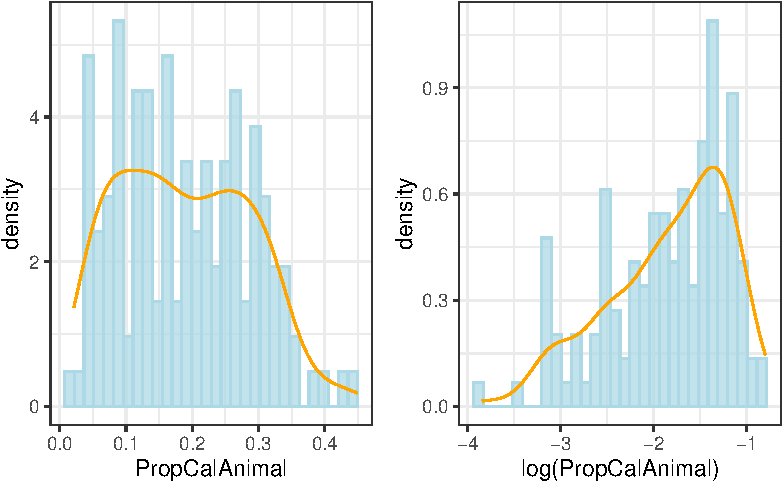
\includegraphics{code_files/figure-pdf/unnamed-chunk-7-1.pdf}

}

\end{figure}

\begin{enumerate}
\def\labelenumi{\arabic{enumi}.}
\setcounter{enumi}{2}
\tightlist
\item
  Estimation result, Correlation of explanatory variables, and
  Homoskedasticity check of model (2):
\end{enumerate}

\begin{Shaded}
\begin{Highlighting}[]
\NormalTok{expl\_vars\_cor }\OtherTok{\textless{}{-}} \FunctionTok{cor}\NormalTok{((data\_02 }\SpecialCharTok{|\textgreater{}}  \FunctionTok{select}\NormalTok{(AgLandShare, AgGdpShare, ArableLandShare, GdpPerCapita, HCI, LifeExp, PopMiddle, PopOld, PopFemale, PopUrban)))}

\FunctionTok{corrplot}\NormalTok{(expl\_vars\_cor,}\AttributeTok{method =} \StringTok{\textquotesingle{}color\textquotesingle{}}\NormalTok{,}\AttributeTok{type =} \StringTok{\textquotesingle{}upper\textquotesingle{}}\NormalTok{, }\AttributeTok{addCoef.col =} \StringTok{\textquotesingle{}black\textquotesingle{}}\NormalTok{, }
         \AttributeTok{title =} \StringTok{"Correlation of Explanatory Variables"}\NormalTok{,}
         \AttributeTok{number.digits =} \DecValTok{1}\NormalTok{,  }\AttributeTok{mar=}\FunctionTok{c}\NormalTok{(}\DecValTok{0}\NormalTok{,}\DecValTok{0}\NormalTok{,}\DecValTok{1}\NormalTok{,}\DecValTok{0}\NormalTok{)}\CommentTok{\#Fix the title position}
\NormalTok{         )}

\NormalTok{model\_02 }\OtherTok{\textless{}{-}} \FunctionTok{lm}\NormalTok{(}\AttributeTok{data =}\NormalTok{ data\_02, }
               \AttributeTok{formula =}\NormalTok{ PropCalAnimal }\SpecialCharTok{\textasciitilde{}}\NormalTok{ AgLandShare }\SpecialCharTok{+}\NormalTok{ AgGdpShare }\SpecialCharTok{+} 
\NormalTok{                 ArableLandShare }\SpecialCharTok{+}\NormalTok{ GdpPerCapita }\SpecialCharTok{+}\NormalTok{ HCI }\SpecialCharTok{+}\NormalTok{ LifeExp }\SpecialCharTok{+}\NormalTok{ PopMiddle }\SpecialCharTok{+}
\NormalTok{                 PopOld }\SpecialCharTok{+}\NormalTok{ PopFemale }\SpecialCharTok{+}\NormalTok{ PopUrban)}

\FunctionTok{stargazer}\NormalTok{(model\_02, }\AttributeTok{type =} \StringTok{"text"}\NormalTok{, }\AttributeTok{font.size =} \StringTok{"footnotesize"}\NormalTok{, }
          \AttributeTok{column.sep.width =} \StringTok{"1pt"}\NormalTok{, }\AttributeTok{single.row =} \ConstantTok{TRUE}\NormalTok{,}
          \AttributeTok{digits=}\DecValTok{2}\NormalTok{, }\AttributeTok{no.space =} \ConstantTok{TRUE}\NormalTok{)}

\FunctionTok{bptest}\NormalTok{(model\_02)}
\end{Highlighting}
\end{Shaded}

\begin{enumerate}
\def\labelenumi{\arabic{enumi}.}
\setcounter{enumi}{2}
\tightlist
\item
  Estimation result and Homoskedasticity check of model (3):
\end{enumerate}

\begin{Shaded}
\begin{Highlighting}[]
\NormalTok{model\_03 }\OtherTok{\textless{}{-}} \FunctionTok{lm}\NormalTok{(}\AttributeTok{data =}\NormalTok{ data\_02, }
               \AttributeTok{formula =} \FunctionTok{log}\NormalTok{(PropCalAnimal) }\SpecialCharTok{\textasciitilde{}}\NormalTok{ AgLandShare }\SpecialCharTok{+}\NormalTok{ AgGdpShare }\SpecialCharTok{+} 
\NormalTok{                 ArableLandShare }\SpecialCharTok{+}\NormalTok{ GdpPerCapita }\SpecialCharTok{+}\NormalTok{ HCI }\SpecialCharTok{+}\NormalTok{ LifeExp }\SpecialCharTok{+}\NormalTok{ PopMiddle }\SpecialCharTok{+}
\NormalTok{                 PopOld }\SpecialCharTok{+}\NormalTok{ PopFemale }\SpecialCharTok{+}\NormalTok{ PopUrban)}

\FunctionTok{stargazer}\NormalTok{(model\_03, }\AttributeTok{type =} \StringTok{"text"}\NormalTok{, }\AttributeTok{font.size =} \StringTok{"footnotesize"}\NormalTok{, }
          \AttributeTok{column.sep.width =} \StringTok{"1pt"}\NormalTok{, }\AttributeTok{single.row =} \ConstantTok{TRUE}\NormalTok{,}
          \AttributeTok{digits=}\DecValTok{2}\NormalTok{, }\AttributeTok{no.space =} \ConstantTok{TRUE}\NormalTok{)}

\FunctionTok{bptest}\NormalTok{(model\_03)}
\end{Highlighting}
\end{Shaded}

\begin{enumerate}
\def\labelenumi{\arabic{enumi}.}
\setcounter{enumi}{3}
\tightlist
\item
  Residual distribution of model (2) and model (3):
\end{enumerate}

\begin{Shaded}
\begin{Highlighting}[]
\NormalTok{res\_model\_02 }\OtherTok{\textless{}{-}} \FunctionTok{ggplot}\NormalTok{(}\AttributeTok{data =} \FunctionTok{data.frame}\NormalTok{(}\AttributeTok{value =} \FunctionTok{residuals}\NormalTok{(model\_02)), }
             \AttributeTok{mapping =} \FunctionTok{aes}\NormalTok{(}\AttributeTok{x =}\NormalTok{ value)) }\SpecialCharTok{+}
  \FunctionTok{geom\_histogram}\NormalTok{(}\AttributeTok{mapping =} \FunctionTok{aes}\NormalTok{(}\AttributeTok{y =}\NormalTok{ ..density..), }
                 \AttributeTok{fill =} \StringTok{"lightblue"}\NormalTok{, }\AttributeTok{color =} \StringTok{"lightblue"}\NormalTok{,}
                 \AttributeTok{alpha =} \FloatTok{0.75}\NormalTok{) }\SpecialCharTok{+}
  \FunctionTok{geom\_density}\NormalTok{(}\AttributeTok{color =} \StringTok{"orange"}\NormalTok{) }\SpecialCharTok{+}
  \FunctionTok{xlab}\NormalTok{(}\StringTok{"Residuals of model (2)"}\NormalTok{) }\SpecialCharTok{+} 
  \FunctionTok{theme\_bw}\NormalTok{()}

\NormalTok{res\_model\_03 }\OtherTok{\textless{}{-}} \FunctionTok{ggplot}\NormalTok{(}\AttributeTok{data =} \FunctionTok{data.frame}\NormalTok{(}\AttributeTok{value =} \FunctionTok{residuals}\NormalTok{(model\_03)), }
             \AttributeTok{mapping =} \FunctionTok{aes}\NormalTok{(}\AttributeTok{x =}\NormalTok{ value)) }\SpecialCharTok{+}
  \FunctionTok{geom\_histogram}\NormalTok{(}\AttributeTok{mapping =} \FunctionTok{aes}\NormalTok{(}\AttributeTok{y =}\NormalTok{ ..density..), }
                 \AttributeTok{fill =} \StringTok{"lightblue"}\NormalTok{, }\AttributeTok{color =} \StringTok{"lightblue"}\NormalTok{,}
                 \AttributeTok{alpha =} \FloatTok{0.75}\NormalTok{) }\SpecialCharTok{+}
  \FunctionTok{geom\_density}\NormalTok{(}\AttributeTok{color =} \StringTok{"orange"}\NormalTok{) }\SpecialCharTok{+} 
  \FunctionTok{xlab}\NormalTok{(}\StringTok{"Residuals of model (3)"}\NormalTok{) }\SpecialCharTok{+} 
  \FunctionTok{theme\_bw}\NormalTok{()}

\NormalTok{res\_model\_02 }\SpecialCharTok{+}\NormalTok{ res\_model\_03}
\end{Highlighting}
\end{Shaded}

\begin{enumerate}
\def\labelenumi{\arabic{enumi}.}
\setcounter{enumi}{4}
\tightlist
\item
  Restricted F-test for model(2) by removing AgLandShare and AgGdpShare
\end{enumerate}

\begin{Shaded}
\begin{Highlighting}[]
\NormalTok{model\_02\_restrict }\OtherTok{\textless{}{-}} \FunctionTok{lm}\NormalTok{(}\AttributeTok{data =}\NormalTok{ data\_02, }
                        \AttributeTok{formula =}\NormalTok{ PropCalAnimal }\SpecialCharTok{\textasciitilde{}}\NormalTok{ ArableLandShare }\SpecialCharTok{+} 
\NormalTok{                          GdpPerCapita }\SpecialCharTok{+}\NormalTok{ HCI }\SpecialCharTok{+}\NormalTok{ LifeExp }\SpecialCharTok{+} 
\NormalTok{                          PopMiddle }\SpecialCharTok{+}\NormalTok{ PopOld }\SpecialCharTok{+}\NormalTok{ PopFemale }\SpecialCharTok{+}\NormalTok{ PopUrban) }

\FunctionTok{anova}\NormalTok{(model\_02\_restrict, model\_02)}
\end{Highlighting}
\end{Shaded}

\begin{enumerate}
\def\labelenumi{\arabic{enumi}.}
\setcounter{enumi}{5}
\tightlist
\item
  Estimation result of model (4):
\end{enumerate}

\begin{Shaded}
\begin{Highlighting}[]
\NormalTok{model\_04 }\OtherTok{\textless{}{-}} \FunctionTok{lm}\NormalTok{(}\AttributeTok{data =}\NormalTok{ data\_02, }
               \AttributeTok{formula =}\NormalTok{ PropCalAnimal }\SpecialCharTok{\textasciitilde{}}\NormalTok{ ArableLandShare }\SpecialCharTok{+} \FunctionTok{log}\NormalTok{(GdpPerCapita) }
               \SpecialCharTok{+}\NormalTok{ HCI }\SpecialCharTok{+}\NormalTok{ LifeExp }\SpecialCharTok{+}\NormalTok{ PopMiddle }\SpecialCharTok{+}\NormalTok{ PopOld }\SpecialCharTok{+}\NormalTok{ PopFemale }\SpecialCharTok{+}\NormalTok{ PopUrban)}

\FunctionTok{stargazer}\NormalTok{(model\_04, }\AttributeTok{type =} \StringTok{"text"}\NormalTok{, }\AttributeTok{font.size =} \StringTok{"footnotesize"}\NormalTok{, }
          \AttributeTok{column.sep.width =} \StringTok{"1pt"}\NormalTok{, }\AttributeTok{single.row =} \ConstantTok{TRUE}\NormalTok{,}
          \AttributeTok{digits=}\DecValTok{2}\NormalTok{, }\AttributeTok{no.space =} \ConstantTok{TRUE}\NormalTok{)}
\end{Highlighting}
\end{Shaded}

\begin{enumerate}
\def\labelenumi{\arabic{enumi}.}
\setcounter{enumi}{6}
\tightlist
\item
  Estimation result of model (4) with Quadratic HCI:
\end{enumerate}

\begin{Shaded}
\begin{Highlighting}[]
\NormalTok{model\_04\_hci\_square }\OtherTok{\textless{}{-}} \FunctionTok{lm}\NormalTok{(}\AttributeTok{data =}\NormalTok{ data\_02, }
               \AttributeTok{formula =}\NormalTok{ PropCalAnimal }\SpecialCharTok{\textasciitilde{}}\NormalTok{ ArableLandShare }\SpecialCharTok{+} \FunctionTok{log}\NormalTok{(GdpPerCapita) }
               \SpecialCharTok{+}\NormalTok{ HCI }\SpecialCharTok{+} \FunctionTok{I}\NormalTok{(HCI}\SpecialCharTok{\^{}}\DecValTok{2}\NormalTok{) }\SpecialCharTok{+}\NormalTok{ LifeExp }\SpecialCharTok{+}\NormalTok{ PopMiddle }\SpecialCharTok{+}\NormalTok{ PopOld }\SpecialCharTok{+}\NormalTok{ PopFemale }\SpecialCharTok{+}\NormalTok{ PopUrban)}

\FunctionTok{stargazer}\NormalTok{(model\_04\_hci\_square, }\AttributeTok{type =} \StringTok{"text"}\NormalTok{, }\AttributeTok{font.size =} \StringTok{"footnotesize"}\NormalTok{, }
          \AttributeTok{column.sep.width =} \StringTok{"1pt"}\NormalTok{, }\AttributeTok{single.row =} \ConstantTok{TRUE}\NormalTok{,}
          \AttributeTok{digits=}\DecValTok{4}\NormalTok{, }\AttributeTok{no.space =} \ConstantTok{TRUE}\NormalTok{)}
\end{Highlighting}
\end{Shaded}

\begin{enumerate}
\def\labelenumi{\arabic{enumi}.}
\setcounter{enumi}{7}
\tightlist
\item
  Complete comparison of models
\end{enumerate}

\begin{Shaded}
\begin{Highlighting}[]
\NormalTok{bp\_test\_model\_02 }\OtherTok{\textless{}{-}} \FunctionTok{bptest}\NormalTok{(model\_02)}
\NormalTok{bp\_test2\_model\_03 }\OtherTok{\textless{}{-}} \FunctionTok{bptest}\NormalTok{(model\_03)}
\NormalTok{bp\_test2\_model\_04 }\OtherTok{\textless{}{-}} \FunctionTok{bptest}\NormalTok{(model\_04)}

\NormalTok{reset\_test\_model\_02 }\OtherTok{\textless{}{-}} \FunctionTok{resettest}\NormalTok{(model\_02, }\AttributeTok{power=}\DecValTok{2}\NormalTok{, }\AttributeTok{type=}\StringTok{"regressor"}\NormalTok{, }\AttributeTok{vcov. =} \FunctionTok{vcovHC}\NormalTok{(model\_02, }\StringTok{"HC1"}\NormalTok{))}
\NormalTok{reset\_test\_model\_03 }\OtherTok{\textless{}{-}} \FunctionTok{resettest}\NormalTok{(model\_03, }\AttributeTok{power=}\DecValTok{2}\NormalTok{, }\AttributeTok{type=}\StringTok{"regressor"}\NormalTok{, }\AttributeTok{vcov. =} \FunctionTok{vcovHC}\NormalTok{(model\_03, }\StringTok{"HC1"}\NormalTok{))}
\NormalTok{reset\_test\_model\_04 }\OtherTok{\textless{}{-}} \FunctionTok{resettest}\NormalTok{(model\_04, }\AttributeTok{power=}\DecValTok{2}\NormalTok{, }\AttributeTok{type=}\StringTok{"regressor"}\NormalTok{, }\AttributeTok{vcov. =} \FunctionTok{vcovHC}\NormalTok{(model\_04, }\StringTok{"HC1"}\NormalTok{))}

\FunctionTok{stargazer}\NormalTok{(model\_02, model\_03, model\_04, }\AttributeTok{type=}\StringTok{"text"}\NormalTok{,}
          \AttributeTok{align=}\ConstantTok{TRUE}\NormalTok{,}
          \AttributeTok{add.lines=}\FunctionTok{list}\NormalTok{(}
            \FunctionTok{c}\NormalTok{(}\StringTok{"BP Test P{-}value"}\NormalTok{, }\FunctionTok{sprintf}\NormalTok{(}\StringTok{"\%.3f"}\NormalTok{, bp\_test\_model\_02}\SpecialCharTok{$}\NormalTok{p.value), }
              \FunctionTok{sprintf}\NormalTok{(}\StringTok{"\%.3f"}\NormalTok{, bp\_test2\_model\_03}\SpecialCharTok{$}\NormalTok{p.value), }
              \FunctionTok{sprintf}\NormalTok{(}\StringTok{"\%.3f"}\NormalTok{, bp\_test2\_model\_04}\SpecialCharTok{$}\NormalTok{p.value)),}
            \FunctionTok{c}\NormalTok{(}\StringTok{"RESET (power=2) Test P{-}value"}\NormalTok{, }\FunctionTok{sprintf}\NormalTok{(}\StringTok{"\%.3f"}\NormalTok{, reset\_test\_model\_02}\SpecialCharTok{$}\NormalTok{p.value), }
              \FunctionTok{sprintf}\NormalTok{(}\StringTok{"\%.3f"}\NormalTok{, reset\_test\_model\_03}\SpecialCharTok{$}\NormalTok{p.value), }
              \FunctionTok{sprintf}\NormalTok{(}\StringTok{"\%.3f"}\NormalTok{, reset\_test\_model\_04}\SpecialCharTok{$}\NormalTok{p.value))}
\NormalTok{          ), }
          \AttributeTok{column.sep.width =} \StringTok{"1pt"}\NormalTok{,}
          \AttributeTok{font.size =} \StringTok{"footnotesize"}
\NormalTok{          )}
\end{Highlighting}
\end{Shaded}

\begin{enumerate}
\def\labelenumi{\arabic{enumi}.}
\setcounter{enumi}{8}
\tightlist
\item
  Model(3) summary with robust-heteroskedasticity standadrd error
\end{enumerate}

\begin{Shaded}
\begin{Highlighting}[]
\NormalTok{cov1 }\OtherTok{=} \FunctionTok{vcovHC}\NormalTok{(model\_03, }\AttributeTok{type =} \StringTok{"HC1"}\NormalTok{)}
\NormalTok{robust\_se }\OtherTok{=} \FunctionTok{sqrt}\NormalTok{(}\FunctionTok{diag}\NormalTok{(cov1))}
\CommentTok{\# Report in stargazer}
\FunctionTok{stargazer}\NormalTok{(model\_03, model\_03, }
          \AttributeTok{type =} \StringTok{"text"}\NormalTok{,}
          \AttributeTok{se =} \FunctionTok{list}\NormalTok{(}\ConstantTok{NULL}\NormalTok{, robust\_se), }\CommentTok{\# setting to robust se}
          \AttributeTok{column.sep.width =} \StringTok{"1pt"}\NormalTok{,}
          \AttributeTok{font.size =} \StringTok{"footnotesize"}\NormalTok{,}
          \AttributeTok{omit.stat =} \FunctionTok{c}\NormalTok{(}\StringTok{"ser"}\NormalTok{, }\StringTok{"F"}\NormalTok{, }\StringTok{"adj.rsq"}\NormalTok{, }\StringTok{"rsq"}\NormalTok{)}
\NormalTok{          )}
\end{Highlighting}
\end{Shaded}




\end{document}
